% arara: xelatex
% arara: xelatex

\documentclass{beamer}
\usepackage{menukeys}
\usepackage{multicol}
\usepackage{mwe}
\usepackage{style}
\usepackage{listings}
\usepackage{smcm-cosc-listings}
\usetikzlibrary{fit,shapes,arrows,arrows.meta}
\usepackage{fontspec}
\setmonofont{Courier}
\setlength\labelsep{1.5ex}
\setlength\fboxsep{1ex}
\usepackage{dirtree}

\usepackage[absolute,overlay]{textpos}

\begin{document}
\begin{frame}[fragile,t]
  \maketitle
  \vspace{1in}
  \begin{columns}[t]
    \begin{column}{.45\textwidth}
      \begin{block}{Abstract}
        In computer science,
            a self-stabilizing algorithm is
            a fault-tolerant problem-solving process that,
            when applied repeatedly to a system,
            will coerce the system into a ‘correct state’.
        Given their parallel nature,
            algorithms of this class are more difficult
            to create and prove correct than
            more traditional, procedural algorithms.
        To aid in further research,
            \st provides an extensible utility for
            the representation, creation, and evaluation
            of self-stabilizing algorithms.
      \end{block}

      \begin{block}{Example \Dash Maximal Independent Set}
        \begin{minipage}[b]{4in}
          \begin{enumerate}
          \item[{\setlength\fboxrule{0pt}\fbox1}]
          \begin{tikzpicture}[baseline=4.5in,scale=1.5]
            \node[graph vertex, marked] (1) at (0 , 3) {$v_1$};
            \node[graph vertex,       ] (2) at (0 , 6) {$v_2$};
            \node[graph vertex,       ] (3) at (3 , 3) {$v_3$};
            \node[graph vertex, marked] (4) at (3 , 6) {$v_4$};
            \node[graph vertex,       ] (5) at (5 , 8) {$v_5$};
      
            \graph {
              (1) -- (3) -- (4) -- (2) --[bend left] (5),
              (1) -- (2),
              (1) -- (4),
              (3) --[bend right] (5)
            };
        \end{tikzpicture}
          \item[{\setlength\fboxrule{0pt}\fbox2}]
          \begin{tikzpicture}[baseline=4.5in,scale=1.5]
            \node[graph vertex, marked] (1) at (0 , 3) {$v_1$};
            \node[graph vertex,       ] (2) at (0 , 6) {$v_2$};
            \node[graph vertex,       ] (3) at (3 , 3) {$v_3$};
            \node[graph vertex, marked] (4) at (3 , 6) {$v_4$};
            \node[graph vertex, marked] (5) at (5 , 8) {$v_5$};
      
            \graph {
              (1) -- (3) -- (4) -- (2) --[bend left] (5),
              (1) -- (2),
              (1) -- (4),
              (3) --[bend right] (5)
            };
        \end{tikzpicture}
          \item[\fbox3]
          \begin{tikzpicture}[baseline=4.5in,scale=1.5]
            \node[graph vertex, marked] (1) at (0 , 3) {$v_1$};
            \node[graph vertex,       ] (2) at (0 , 6) {$v_2$};
            \node[graph vertex,       ] (3) at (3 , 3) {$v_3$};
            \node[graph vertex,       ] (4) at (3 , 6) {$v_4$};
            \node[graph vertex, marked] (5) at (5 , 8) {$v_5$};
      
            \graph {
              (1) -- (3) -- (4) -- (2) --[bend left] (5),
              (1) -- (2),
              (1) -- (4),
              (3) --[bend right] (5)
            };
        \end{tikzpicture}
          \end{enumerate}
        \end{minipage}
        \hfill
        \begin{minipage}[b]{9in}
          \newcommand\fOf[1]{f\,(#1\,)}
          \centerline{\IndSet}
          \vspace{2ex}
\begin{lstlisting}[language=ssa,frame=lines]
local $f$

privilege ENTER
  if $\fOf{i} = 0 \land \ForAll{j \in \OpenNeighborhood{i}}{\fOf{j} = 0}$
  then:
    $\fOf{i} = 1$

privilege LEAVE
  if $\fOf{i} = 1 \land \Exists{j \in \OpenNeighborhood{i}}{\fOf{j} = 1}$
  then:
    $\fOf{i} = 0$
\end{lstlisting}
          \vspace{1in}
          The algorithm for maximal independent set consists of two possible privileges:
          \bigskip
          \begin{description}[\texttt{ENTERMMM}]
          \item[\texttt{ENTER}] Not marked and \emph{no} neighbor marked
          \item[\texttt{LEAVE}] Marked and \emph{any} neighbor marked
          \end{description}
          \bigskip
          If either statement is true for any node $v_i$,
            that privilege is `present' on $v_i$
            and $v_i$ could move.
          A privileged node is arbitrarily chosen to make its move,
            after which all privileges are re-evaluated.
          \vspace*{.75in}
        \end{minipage}
      \end{block}

      \begin{block}{Definition}
        A distributed algorithm is called \textit{self-stabilizing} if
        the algorithm coerces the graph into a correct state after a
        \emph{finite} number of moves.  Specifically, they have two properties:
        \begin{description}[algorithmMMMM]
        \item[convergence] The algorithm stops after a finite number of moves.
        \item[closure] The algorithm stops if and only if the state is legitimate.
        \end{description}
        To effect this, we consider a sparse, connected graph of state machines where
          the algorithm is defined either in a central daemon or within each state machine:
        \begin{description}[algorithmMMMM]
        \item[predicate] $\Function[f]{v, N(\!v)}{\SetBoolean}$
        \item[move] new state for $v$
        \item[rule] $\Function[R]{P}{M}$
        \item[algorithm] $\Set{\QuickSequence{R}}$
        \end{description}
        \begin{center}
        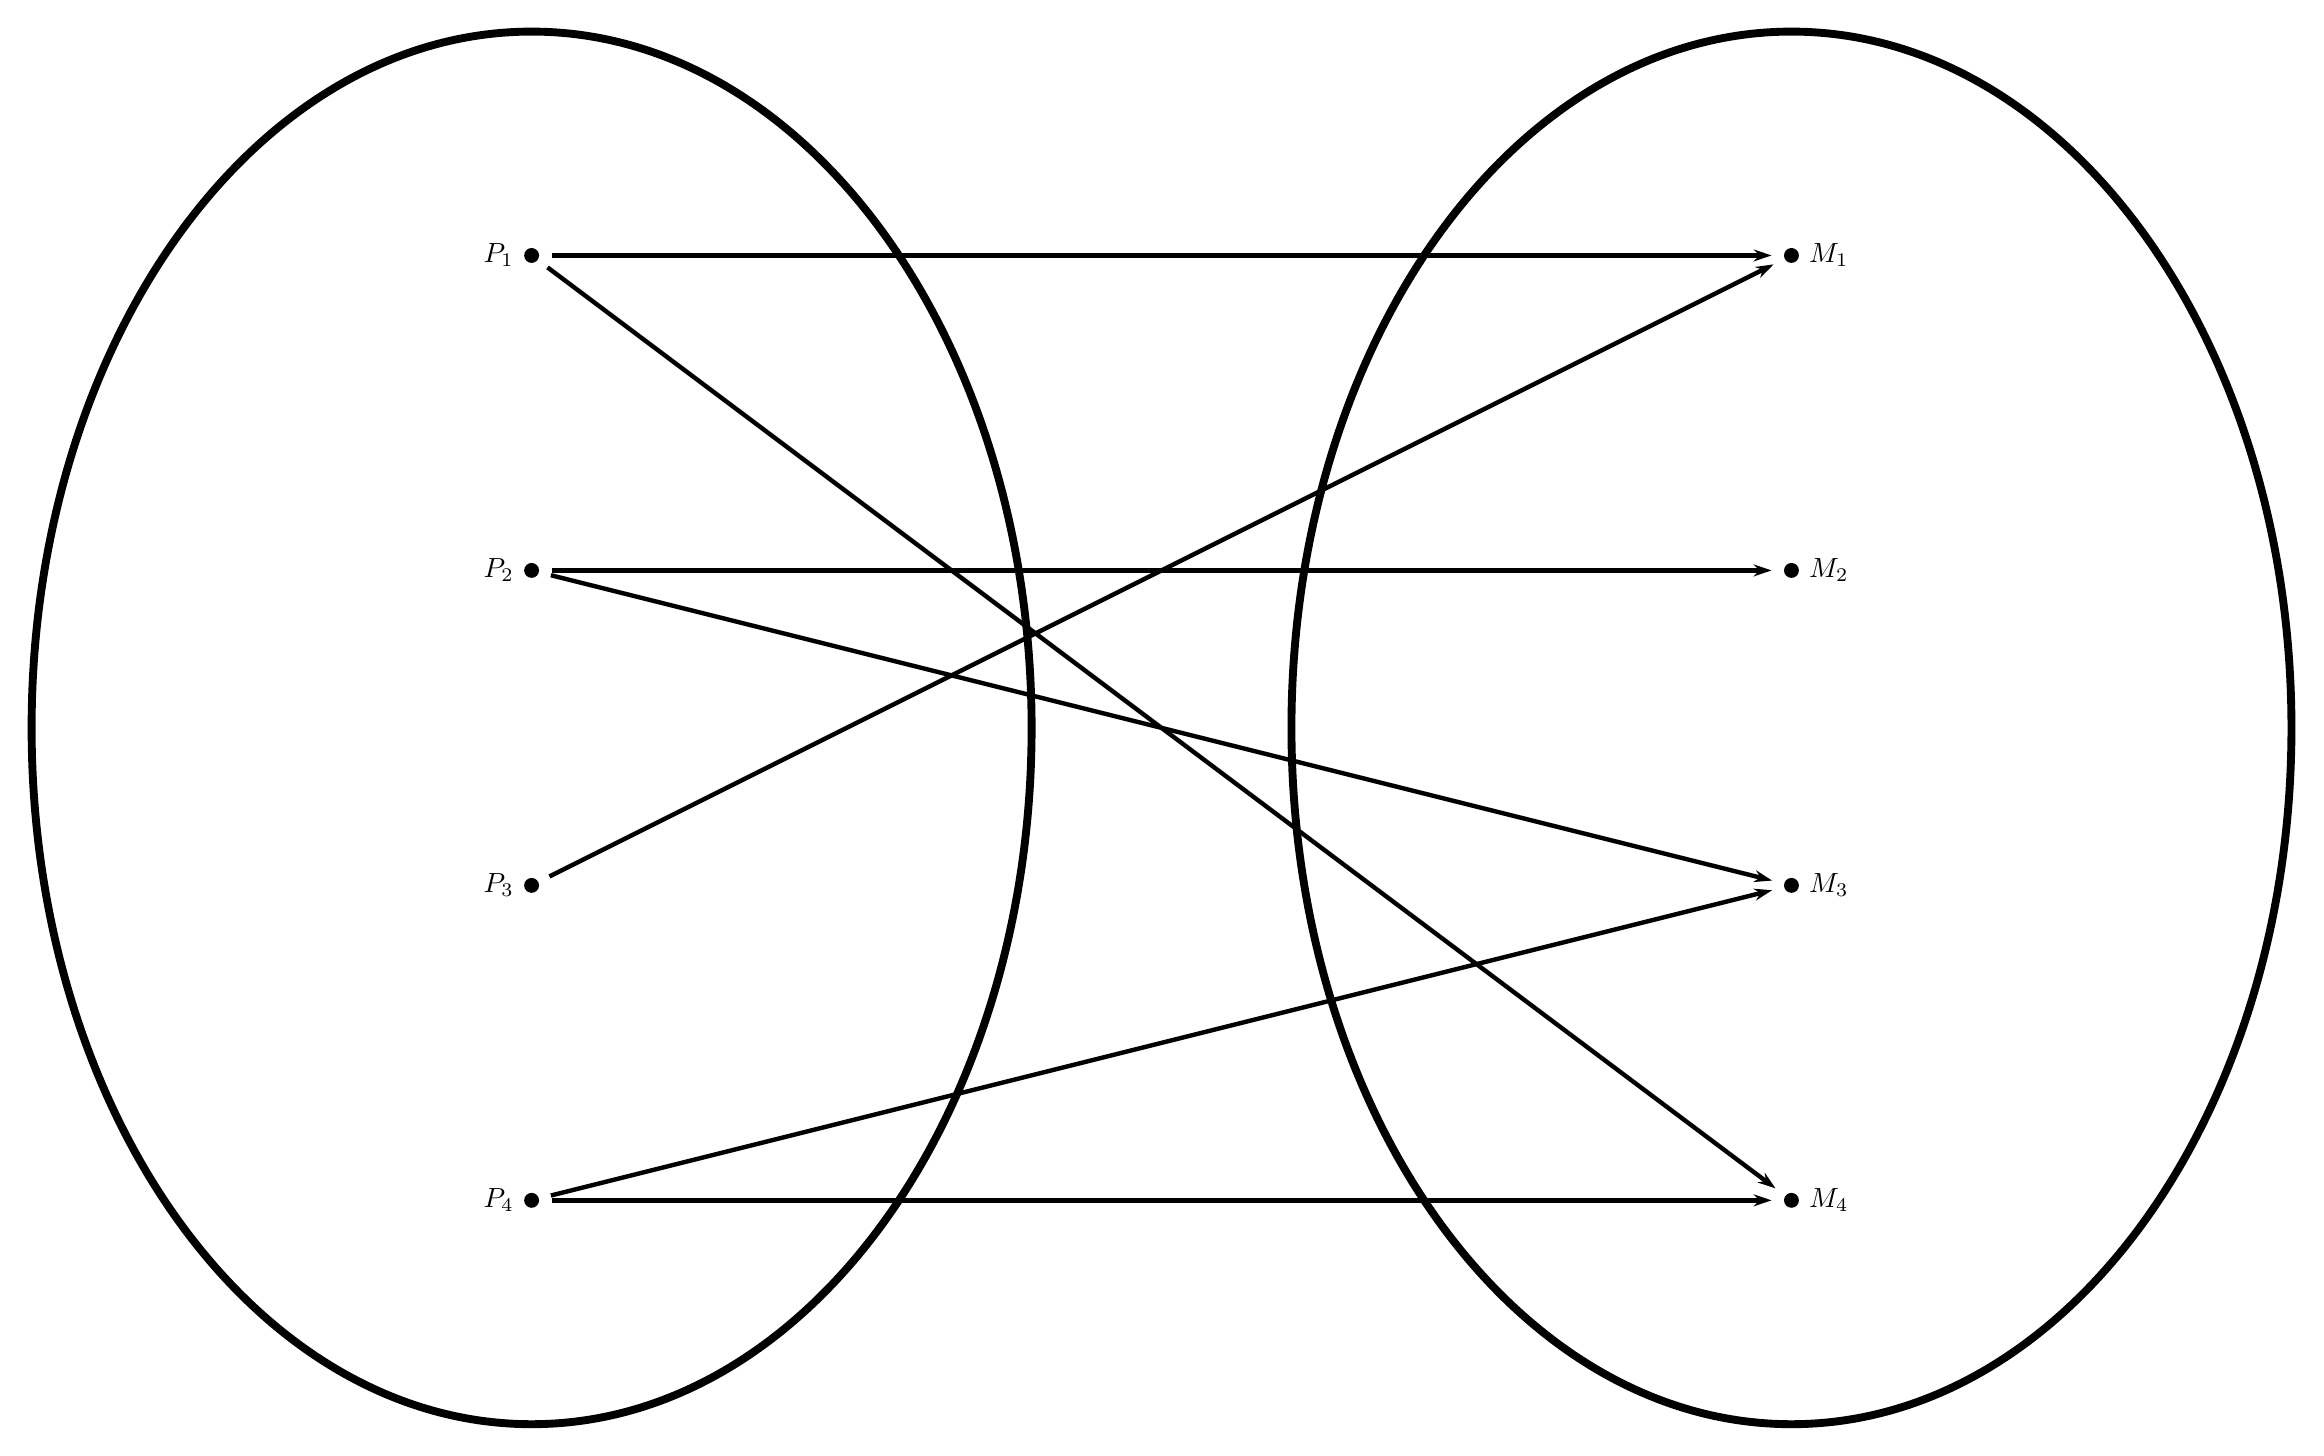
\begin{tikzpicture}[scale=4,
          >=stealth,
          bullet/.style={
            fill=black,
            circle,
            minimum width=1.25ex,
            inner sep=1pt
          },
          projection/.style={
            -{Stealth[width=1ex,length=1.5ex]},
            ultra thick,
            shorten <=1ex,
            shorten >=1ex,
          },
          every fit/.style={
            ellipse,
            line width=1mm,
            draw,
            inner sep=1ex
          }
          ]
          \foreach \y/\l in {1/4,2/3,3/2,4/1} {
            \node[bullet,label=left:$P_\l$] (p\l) at (0,\y) {};
            \node[bullet,label=right:$M_\l$] (m\l) at (4,\y) {};
          }
          
          \node[draw,fit=(p1) (p2) (p3) (p4),minimum width=5in] {} ;
          \node[draw,fit=(m1) (m2) (m3) (m4),minimum width=5in] {} ;
          
          \draw[projection] (p1) -- (m1);
          \draw[projection] (p1) -- (m4);
          \draw[projection] (p2) -- (m2);
          \draw[projection] (p2) -- (m3);
          \draw[projection] (p3) -- (m1);
          \draw[projection] (p4) -- (m4);
          \draw[projection] (p4) -- (m3);
        \end{tikzpicture}
        \end{center}
        \vspace{-.03in}
      \end{block}
      \begin{block}{Further Work}
        \begin{multicols}{2}
          \begin{itemize}
          \item integrated graph creation
          \item integrated test visualization
          \item integration of test cases into `bundle' format
          \item alternative run modes
          \item parallelization of execution
          \item API implemented as successive shell calls
          \end{itemize}
        \end{multicols}%
        \vspace*{-.04in}%
      \end{block}
    \end{column}
    \begin{column}{.45\textwidth}
      \begin{block}{The Bundle Format}
        To store these algorithms on disk, \st uses a two-fold approach:
        \begin{itemize}
        \item A series of YAML documents is maintained to provide
          metadata for the basic entities as well as depict the
          relationships between those entities
        \item Basic components (predicates\slash moves) are maintained
          without repetition in a predetermined, configurable
          directory structure
        \end{itemize}
        Under this structure, \IndSet would look similar to the following
          (with much more metadata):

        \vspace{-.14in}

        \begin{minipage}{\linewidth}
          \hfill
          \begin{minipage}{5in}
\begin{lstlisting}[language=yaml,basicstyle=\ttfamily\YAMLkeystyle]
--- !Move
name: mark
filename: mark.py
--- !Move
name: unmark
filename: unmark.py
--- !Predicate
name: enter
filename: enter.py
--- !Predicate
name: leave
filename: leave.py
--- !Algorithm
name: Independent Set
rules:
  - !Rule
    predicate: enter
    moves: [ mark ]
  - !Rule
    predicate: leave
    moves: [ unmark ]
\end{lstlisting}
          \end{minipage}
          \hfill
          \begin{minipage}{4in}
            \dirtree{%
              .1 ind-set.ssax/.
              .2 bundle.yaml.
              .2 predicates/.
              .3 enter.py.
              .3 leave.py.
              .2 moves/.
              .3 mark.py.
              .3 unmark.py.
            }
          \end{minipage}
          \hfill
          ~
        \end{minipage}

        with all necessary files, such as \directory{predicates/enter.py}
        \vspace{.3in}
\begin{lstlisting}[language=Python,stringstyle=\color{green!50!black},keywordstyle=\color{blue}]
  marked = v['marked']
  neighbor_marked = any(map(lambda n: n['marked'], N))
  return not (marked or neighbor_marked)
\end{lstlisting}
      \end{block}
      
      \begin{block}{Interface and Architecture}
        \vspace*{-.1ex}

        \setlength\fboxsep{0pt}
        \setlength\fboxrule{.1ex}
        \fcolorbox{black!50}{black!50}{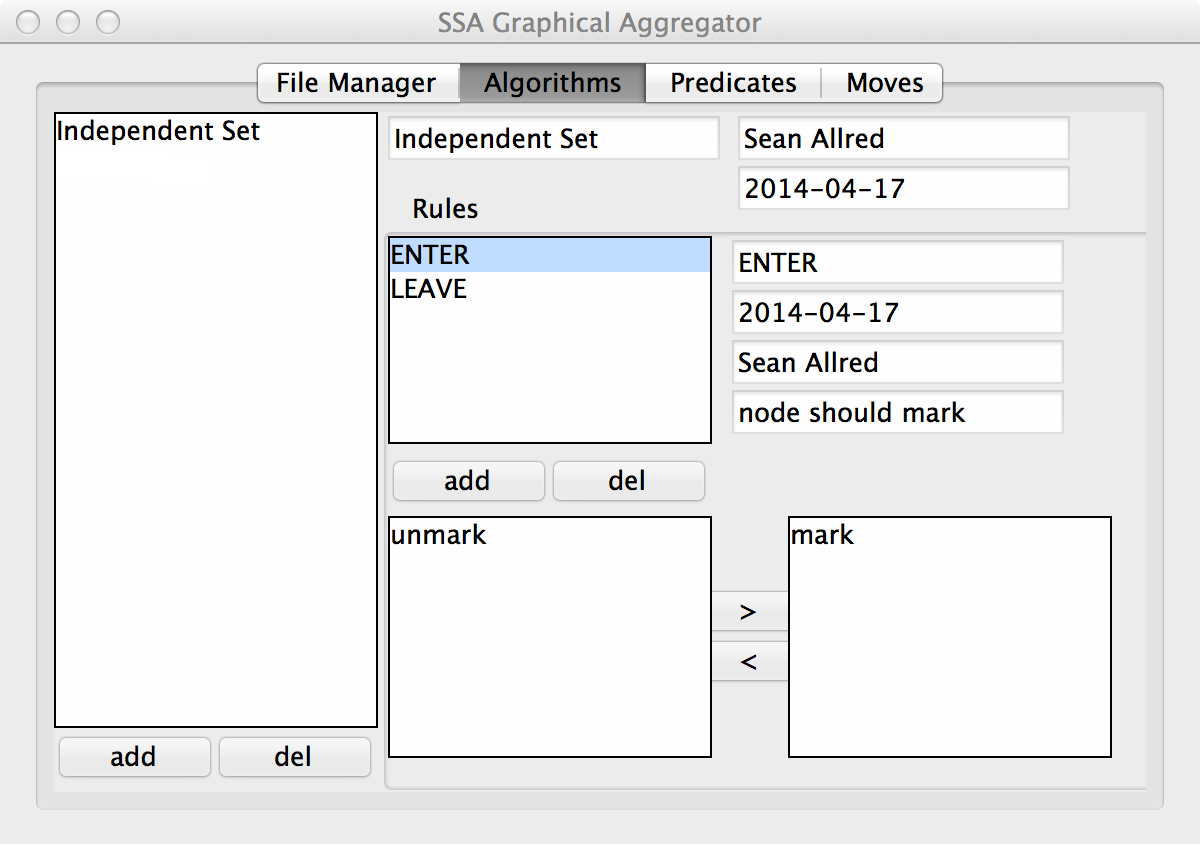
\includegraphics[width=.49\linewidth]{../figs/4}}
        \hfill
        \fcolorbox{black!50}{black!50}{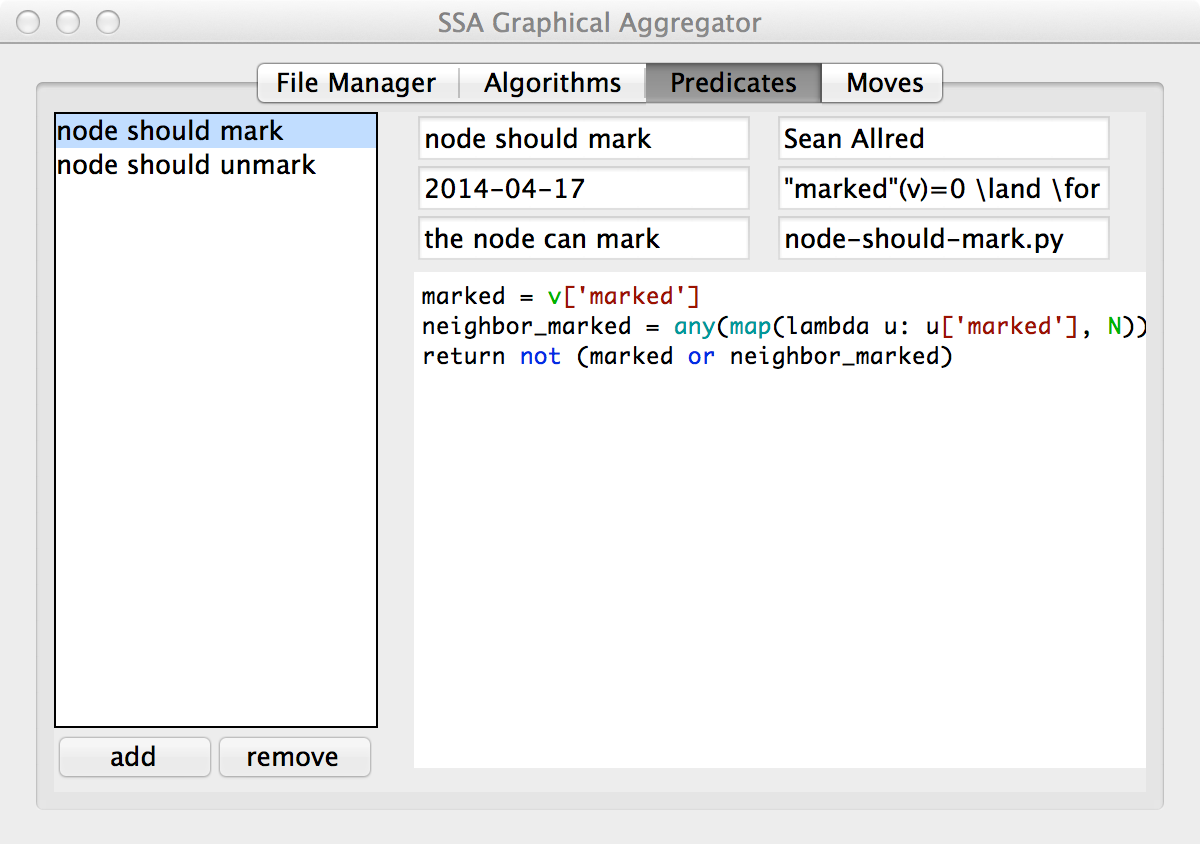
\includegraphics[width=.49\linewidth]{../figs/2}}

        \vspace*{-.1ex}

        Written and tested completely in Python~3 and Tkinter,
          \st not only provides an engine to load and
          run these algorithms on externally-created graphs,
          but also provides a basic graphical interface
          to construct `bundles' \Dash collections of algorithms
          and the necessary components to run them.
          \begin{center}
        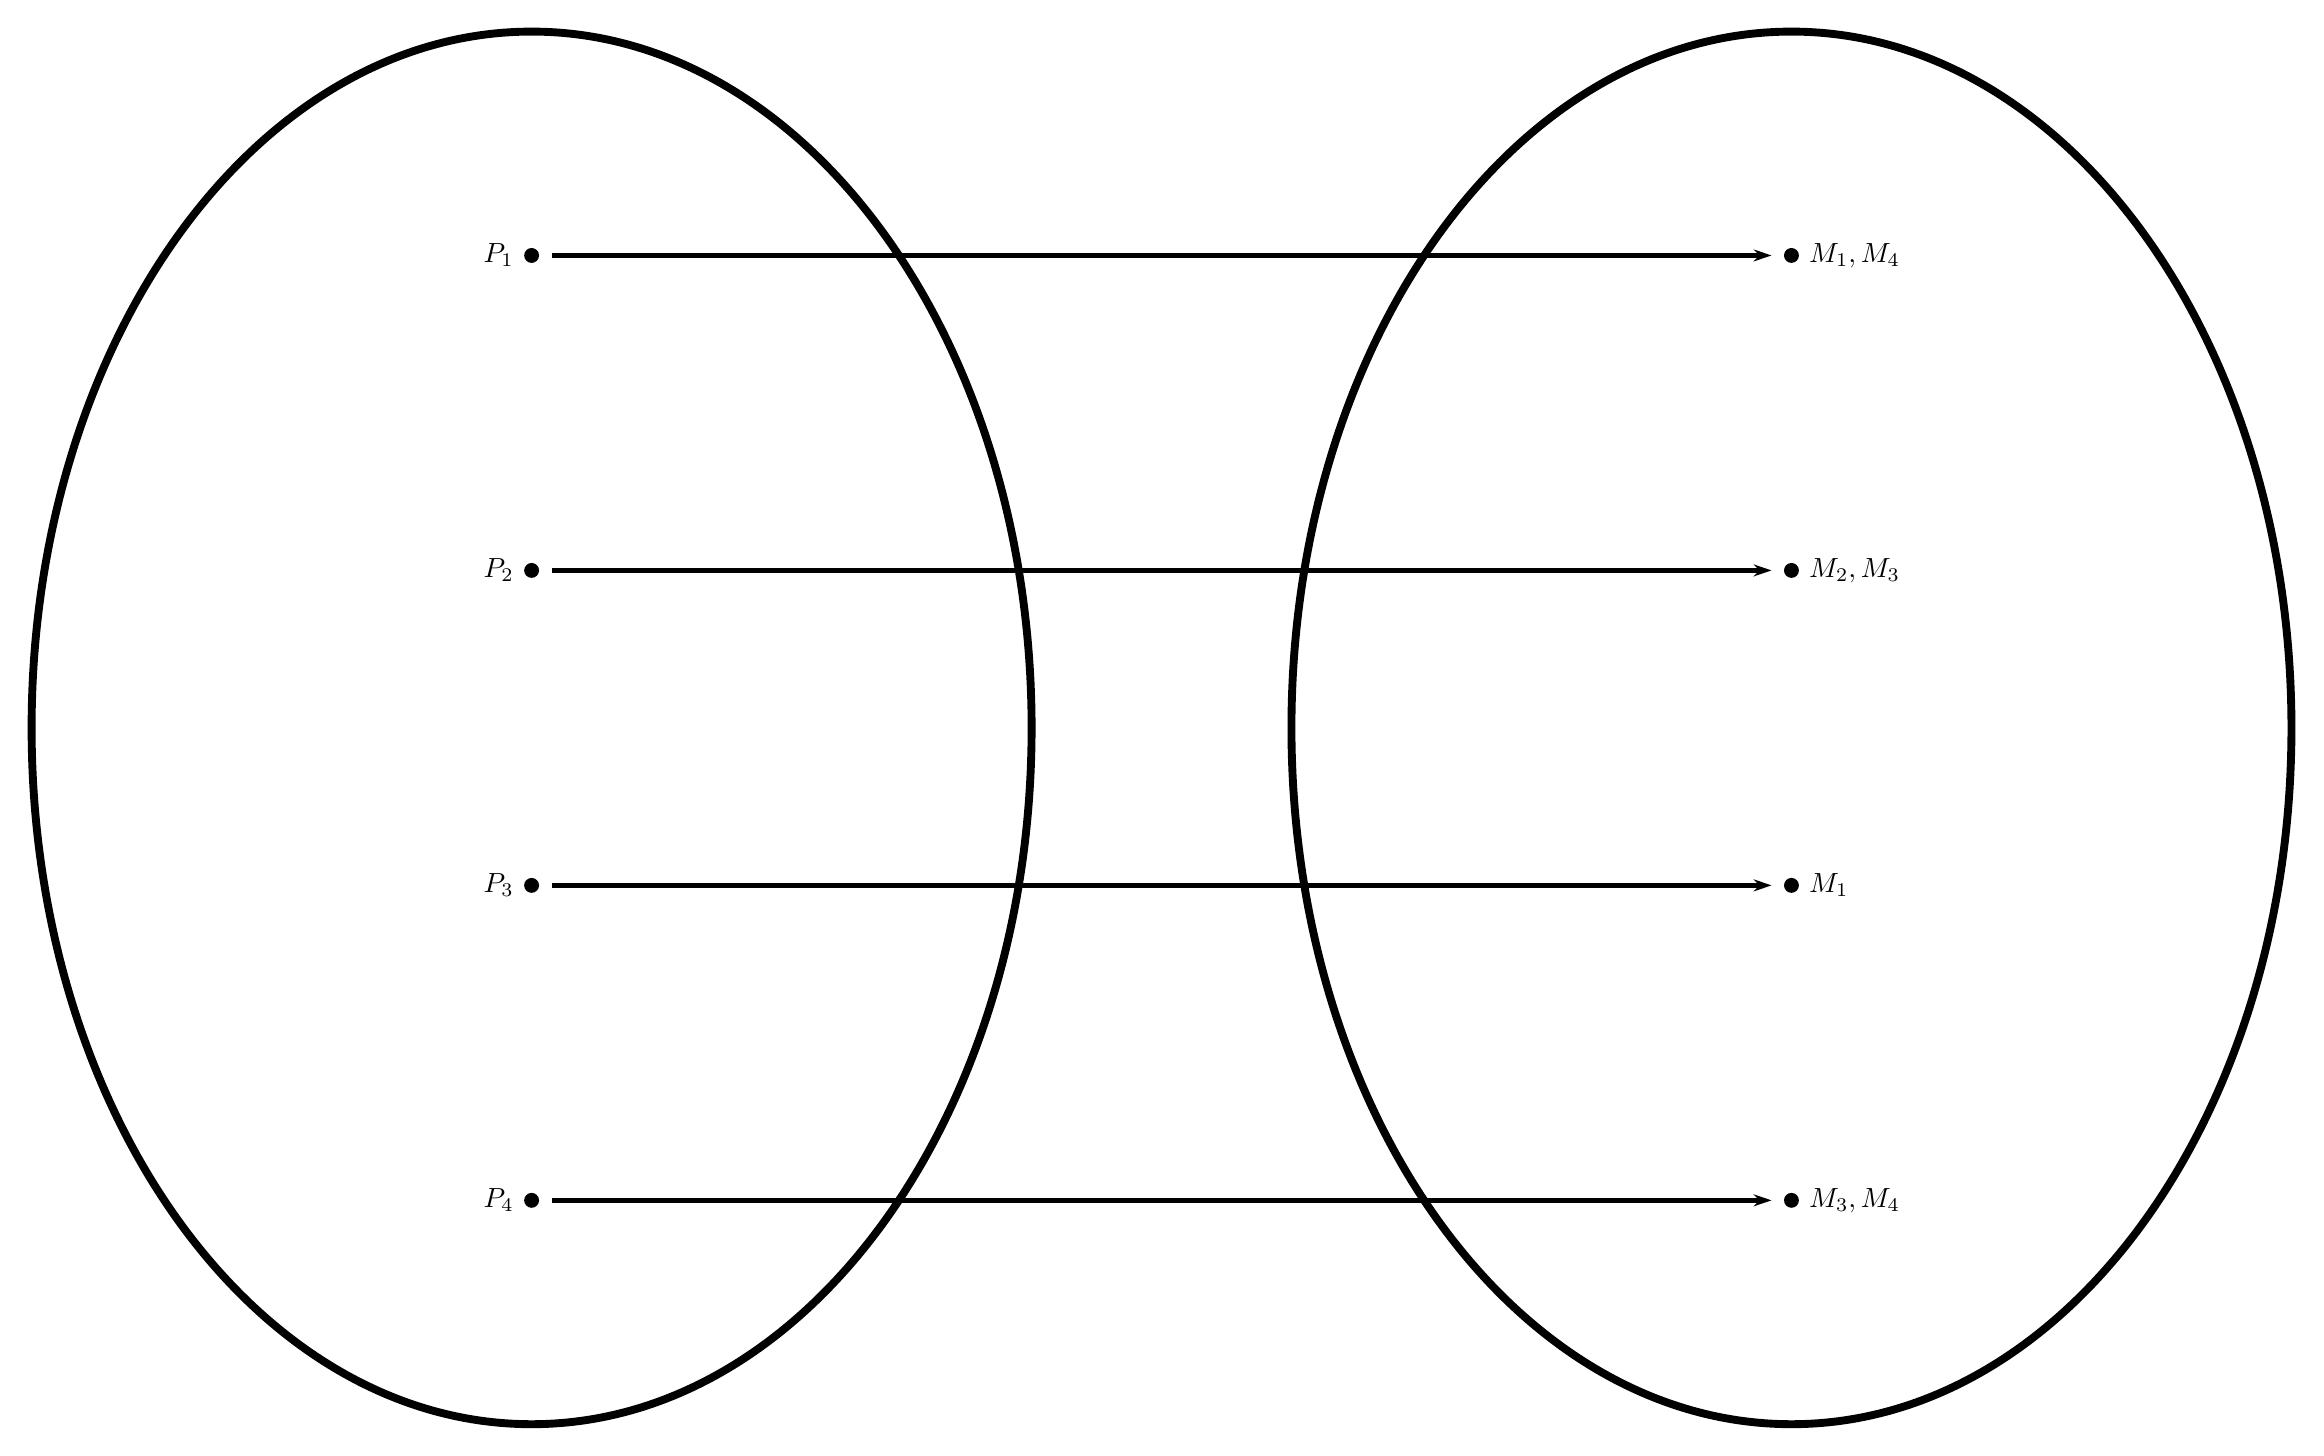
\begin{tikzpicture}[scale=4,
          >=stealth,
          bullet/.style={
            fill=black,
            circle,
            minimum width=1.25ex,
            inner sep=1pt
          },
          projection/.style={
            -{Stealth[width=1ex,length=1.5ex]},
            ultra thick,
            shorten <=1ex,
            shorten >=1ex,
          },
          every fit/.style={
            ellipse,
            line width=1mm,
            draw,
            inner sep=1ex
          }
          ]
          \foreach \y/\l in {1/4,2/3,3/2,4/1} {
            \node[bullet,label=left:$P_\l$] (p\l) at (0,\y) {};
          }

          \node[bullet,label=right:$\Set{M_3,M_4}$] (m4) at (4,1) {};
          \node[bullet,label=right:$\Set{M_1}$] (m3) at (4,2) {};
          \node[bullet,label=right:$\Set{M_2,M_3}$] (m2) at (4,3) {};
          \node[bullet,label=right:$\Set{M_1,M_4}$] (m1) at (4,4) {};
          
          \node[draw,fit=(p1) (p2) (p3) (p4),minimum width=5in] {} ;
          \node[draw,fit=(m1) (m2) (m3) (m4),minimum width=5in] {} ;
          
          \draw[projection] (p1) -- (m1);
          \draw[projection] (p2) -- (m2);
          \draw[projection] (p3) -- (m3);
          \draw[projection] (p4) -- (m4);
        \end{tikzpicture}
          \end{center}
        Care was taken to adhere to the mathematical definitions
          as strictly as possible.
        An important exception is depicted above;
          instead of implementing the design that
          is obvious from the mathematical definition,
          the equivalent design using \emph{dictionaries}
          decreases the memory overhead of the state
          of the algorithm itself.

        \vspace{.16in}

        The algorithm can be run a set number of times or continuously
        until stabilization (or process termination).  As the
        algorithm runs, a log is kept of changes to the graph.  When
        the process completes, these changes are returned as a
        custom-made \texttt{AnimatedGraph} object that can traverse
        the entire history of the graph frame-by-frame.
      \end{block}
    \end{column}
  \end{columns}
\end{frame}
\end{document}

%%% Local Variables:
%%% mode: latex
%%% TeX-master: t
%%% TeX-PDF-mode: t
%%% TeX-command-default: "arara"
%%% truncate-lines: nil
%%% TeX-engine: xetex
%%% End:
